\section*{Задание}
\addcontentsline{toc}{section}{Задание}

Разработать средствами MPI параллельную программу решения уравнения
прямоугольной мембраны методом конечных разностей с использованием явной
вычислительной схемы. Временной интервал моделирования и количество (кратное 8)
узлов по осям $x$ и $y$ расчетной сетки - параметры программы. Уравнение мембраны
имеет следующий вид:

\begin{equation}
    \frac{d^2z}{dt^2} = a^2*(\frac{d^2z}{dx^2}+\frac{d^2z}{dy^2})+f(x,y,t),
    \label{eq:membrane}
\end{equation}


где $t$ - время, $x$, $y$ - пространственные координаты, $z$ - отклонение (малое)
точки мембраны от положения покоя, a - фазовая скорость, $f(x,y,t)$ - внешнее
"силовое" воздействие на мембрану перпендикулярное ее плоскости. Предусмотреть
возможность задания ненулевых начальных условий и ненулевого внешнего
воздействия. Количество элементов в сетке, временной интервал моделирования и
количество параллельных процессов - параметры программы. Программа должна
демонстрировать ускорение по сравнению с последовательным вариантом.
Предусмотреть визуализацию результатов посредством утилиты \texttt{gnuplot}. При этом
утилита \texttt{gnuplot} должна вызываться отдельной командой после окончания расчета.

\newpage

\section*{Описание структуры программы}

\addcontentsline{toc}{section}{Описание структуры программы}

Проект использует 3 библиотеки для отображения работы: 

\begin{itemize}
    \item \texttt{heatmap} для генерации карты отклонения мембраны,
    \item \texttt{lodepng} для генерации рисунка финального кадра
    \item \texttt{gif} для генерации анимации того, как изменяется мембрана под действием внешнего воздействия.
\end{itemize}

Помимо этого, программа разбита на 3 файла: для работы с матрицей, конфигурацией
и mpi.

Матрица представляет собой <<плоский>> массив размером $w * h$, где $w$ - ширина
матрицы, а $h$ - высота. Это сделано для оптимизации доступа, так как в
привычном варианте приходится разыменовывать 2 указателя вместо одного.

В качетстве решателя уравнения (\ref{eq:membrane}) применяются методы конечных
разностей, поэтому в программе хранится сразу 3 состояния мембраны: на текущем,
предыдущем и следующем временных слоях. 

Также, чтобы распараллелить работу
программы, матрица делится на несколько зон под каждый процесс MPI. Каждой такой
зоне нужно дополнительно знать о соседних с нею клетках. Поэтому дополнительно
нужно синхронизировать и соседние зоны в одном MPI процессе (см рис.
\ref{fig:processes}).

\begin{figure}[H]
    \centering
    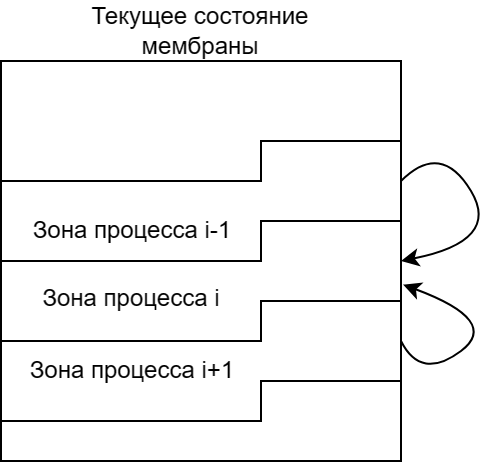
\includegraphics[width=0.6\textwidth]{images/lab4_processes.drawio.png}
    \caption{Разделение матрицы состояния мембраны на зоны}
    \label{fig:processes}
\end{figure}

После рассчета всех временных слоев в каждой зоне, программа генерирует,
используя библиотеку \texttt{gif}, из сохраненных состояний анимацию изменения мембраны.

\newpage

\section*{Блок-схема программы}
\addcontentsline{toc}{section}{Блок-схема программы}

\begin{figure}[H]
    \centering
    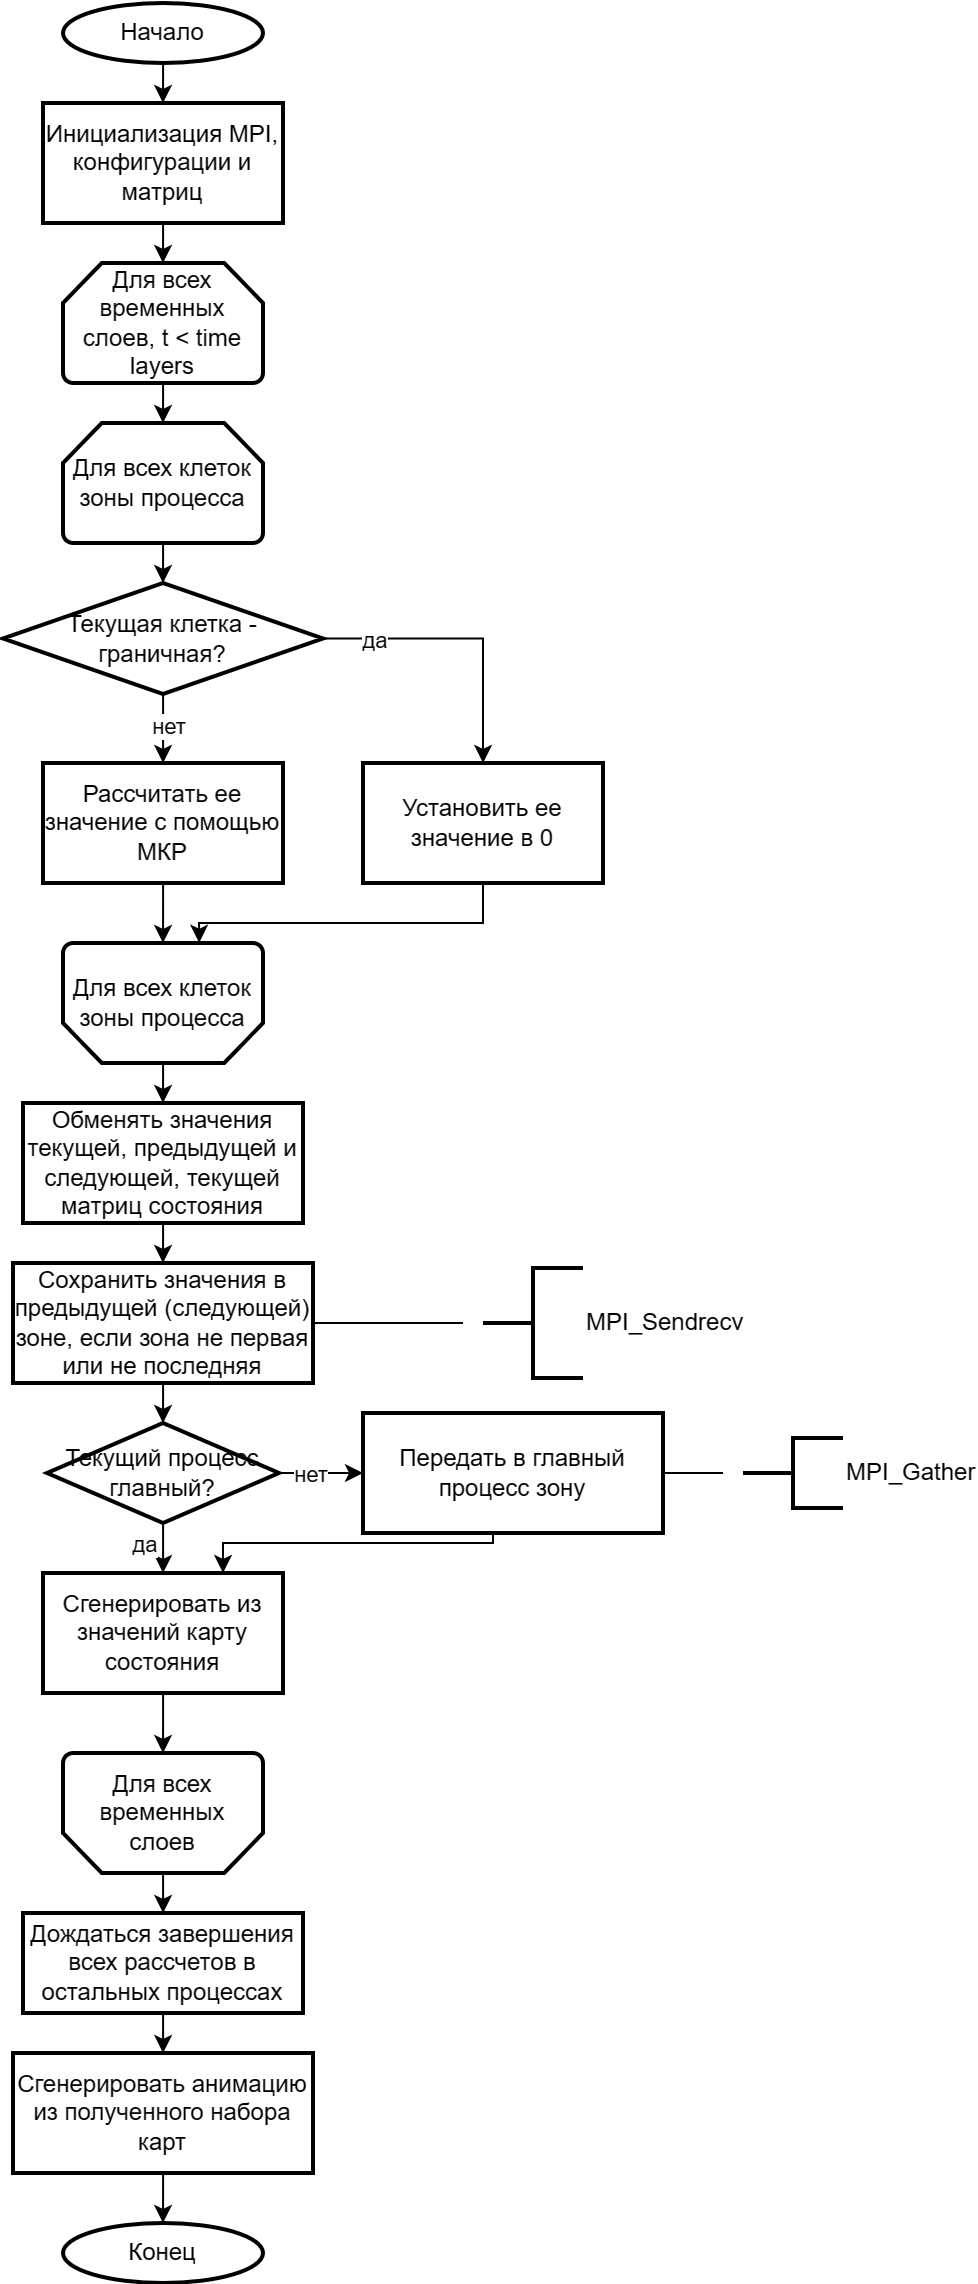
\includegraphics[height=\textheight]{images/lab4_blockscheme.drawio.png}
    \caption{Блок-cхема работы одного из процессов MPI, где в комментарии вынесены используемые функции MPI}
    \label{fig:flowchart}
\end{figure}

\newpage

\section*{Результат работы}
\addcontentsline{toc}{section}{Результат работы}

Программа после выполнения создает 2 файла: один с анимацией состояния мембраны,
другой - изображение ее финального состояния.

Например, если в качестве внешнего воздействия выбрать функцию
(\ref{eq:external}), воздействующую на центр мембраны, то для 100 временных
слоев получится следующее изображение (см. рис. \ref{fig:image})

\begin{equation}
    f(x, y, t) = sin(t + x * y)
    \label{eq:external}
\end{equation}

\begin{figure}[H]
    \centering
    
\includegraphics[width=\linewidth]{images/output.png}
    \caption{Отображение мембраны на плоскости, где цвет показывает высоту каждой клетки}
    \label{fig:image}
\end{figure}

Если в качестве граничных условий выбрать 1, то получится следующее изображение:

\begin{figure}[H]
    \centering
    
\includegraphics[width=\linewidth]{images/output2.png}
    \caption{Отображение мембраны на плоскости, где цвет показывает высоту каждой клетки}
    \label{fig:dsp}
\end{figure}

\newpage

\appendix

\section*{Приложение}
\section*{Текст программы}
\addcontentsline{toc}{section}{Текст программы}

\textbf{include/config.h}

\begin{lstlisting}[
    language=C++,
    directivestyle={\color{black}}, 
    emph={int,char,double,float,unsigned}, 
    emphstyle={\color{blue}}]
    #pragma once

    #include <stdbool.h>
    
    typedef struct {
        bool generateImage;
        int height;
        int width;
        double time_layers;
        double external_weight;
        double a;
        double step;
    } Config;
    
    Config readConfig(int argc, char **argv);
\end{lstlisting}

\textbf{include/matrix.h}

\begin{lstlisting}[
    language=C++,
    directivestyle={\color{black}}, 
    emph={int,char,double,float,unsigned}, 
    emphstyle={\color{blue}}]
    #pragma once

    typedef struct {
        int width, height;
        double *buffer;
    } Matrix;
    
    Matrix newMatrix(int x, int y);
    
    double *get(Matrix m, int x, int y);
    
    double *buffer(Matrix m);
    
    heatmap_t *intoHeatmap(Matrix m);
    
    void freeMatrix(Matrix m);
\end{lstlisting}

\textbf{include/config.c}

\begin{lstlisting}[
    language=C++,
    directivestyle={\color{black}}, 
    emph={int,char,double,float,unsigned}, 
    emphstyle={\color{blue}}]
    #include "config.h"

    Config readConfig(int argc, char **argv) {
        Config empty = {.width = 500,
                        .height = 500,
                        .a = 1,
                        .external_weight = 1,
                        .time_layers = 100,
                        .generateImage = true,
                        .step = 1};
        return empty;
    }
\end{lstlisting}

\textbf{include/matrix.c}

\begin{lstlisting}[
    language=C++,
    directivestyle={\color{black}}, 
    emph={int,char,double,float,unsigned}, 
    emphstyle={\color{blue}}]
    #include <heatmap.h>
    #include <math.h>
    #include <stdlib.h>
    
    #include "matrix.h"
    
    Matrix newMatrix(int x, int y) {
        Matrix m;
        m.width = y;
        m.height = x;
        m.buffer = calloc(x * y, sizeof(double));
        return m;
    }
    
    double *get(Matrix m, int x, int y) { return &m.buffer[x * m.width + y]; }
    
    double *buffer(Matrix m) { return m.buffer; }
    
    heatmap_t *intoHeatmap(Matrix m) {
        heatmap_t *frame = heatmap_new(m.width, m.height);
    
        for (int i = 0; i < m.width; i++)
            for (int j = 0; j < m.height; j++)
                heatmap_add_weighted_point(frame, i, j, fmax(*get(m, i, j), 0));
    
        return frame;
    }
    
    void freeMatrix(Matrix m) { free(m.buffer); }
\end{lstlisting}

\textbf{src/main.c}

\begin{lstlisting}[
    language=C++,
    directivestyle={\color{black}}, 
    emph={int,char,double,float,unsigned}, 
    emphstyle={\color{blue}}]
    #include <math.h>
    #include <signal.h>
    #include <stdio.h>
    #include <stdlib.h>
    #include <sys/time.h>
    #include <unistd.h>
    
    #include <mpi.h>
    #include <pthread.h>
    #include <sched.h>
    #include <string.h>
    
    #include <gif.h>
    #include <heatmap.h>
    #include <lodepng.h>
    
    #include "config.h"
    #include "matrix.h"
    
    Config config;
    
    typedef struct {
        int size;
        int start;
        int end;
        int position;
        int x;
        int y;
        double *top;
        double *down
    } Stripes;
    
    double external(double x, double y, double t) {
        if (x == config.width / 2 && y == config.height / 2) {
            return config.external_weight * sin(x * y + t);
        }
        return 0;
    }
    
    double *getS(Stripes s, Matrix m, int x, int y) {
        int newPos = x * config.width + y;
        if (newPos < s.start)
            return &s.top[s.size - newPos + s.position];
        if (newPos > s.end)
            return &s.down[newPos - s.size];
        return get(m, x, y);
    }
    
    void explicit_solver(Stripes stripes, double t, Matrix current, Matrix prev,
                         Matrix next) {
        int x = stripes.x, y = stripes.y;
        double dx = 1;
        double dy = 1;
        double dt = dx * dy / 2 / config.a;
        double weight = external(stripes.x, stripes.y, t);
    
        /**
         *      C
         *      |
         * B -- A -- D
         *      |
         *      E
         */
    
        double A = *get(current, x, y), B = *getS(stripes, current, x - 1, y);
        double C = *getS(stripes, current, x, y + 1),
               D = *getS(stripes, current, x + 1, y);
        double E = *getS(stripes, current, x, y - 1);
    
        double dzx = (D - 2 * A + B) / dx / dx;
        double dzy = (E - 2 * A + C) / dy / dy;
    
        double dzxy = config.a * config.a * (dzx + dzy) + weight;
        double Ap = *get(prev, x, y);
        double An = *get(next, x, y);
    
        *get(next, x, y) = (-dt * dt * dzxy + Ap + A) / 2;
    }
    
    int main(int argc, char *argv[]) {
        int threads, currentRank;
        MPI_Init(&argc, &argv);
        MPI_Comm_size(MPI_COMM_WORLD, &threads);
        MPI_Comm_rank(MPI_COMM_WORLD, &currentRank);
    
        config = readConfig(argc, argv);
    
        const int height = config.height;
        const int width = config.width;
        const int num_points = height * width;
        const int time_steps = config.time_layers;
        const double a = config.a;
    
        Matrix previous = newMatrix(width, height);
        Matrix current = newMatrix(width, height);
        Matrix next = newMatrix(width, height);
    
        Matrix global = newMatrix(width, height);
    
        heatmap_t *frames[time_steps];
        float last_max = 0;
    
        int offset = num_points / threads;
        int start = offset * currentRank;
        int end = offset * (currentRank + 1);
        int size = offset;
    
        double topStripe[size];
        double downStripe[size];
    
        for (int t = 0; t < time_steps; t++) {
            for (int i = start; i < end; i++) {
                int x = i % width;
                int y = i / width;
    
                if (x == 0 || y == 0 || x == width - 1 || y == height - 1)
                    *get(next, x, y) = 1;
                else {
                    Stripes s = {.x = x,
                                 .y = y,
                                 .start = start,
                                 .end = end,
                                 .position = i,
                                 .top = topStripe,
                                 .down = downStripe};
                    explicit_solver(s, t, current, previous, next);
                }
            }
    
            memmove(buffer(previous), buffer(current), num_points * sizeof(double));
            memmove(buffer(current), buffer(next), num_points * sizeof(double));
    
            if (currentRank != 0)
                MPI_Sendrecv(buffer(current) + start - size, size, MPI_DOUBLE,
                             currentRank - 1, 0, downStripe, size, MPI_DOUBLE,
                             currentRank - 1, MPI_ANY_TAG, MPI_COMM_WORLD,
                             MPI_STATUS_IGNORE);
    
            if (currentRank != threads - 1)
                MPI_Sendrecv(buffer(current) + end, size, MPI_DOUBLE,
                             currentRank + 1, 0, topStripe, size, MPI_DOUBLE,
                             currentRank + 1, MPI_ANY_TAG, MPI_COMM_WORLD,
                             MPI_STATUS_IGNORE);
    
            if (currentRank != 0)
                MPI_Gather(buffer(previous) + start, size, MPI_DOUBLE,
                           buffer(global) + start, size, MPI_DOUBLE, 0,
                           MPI_COMM_WORLD);
            else
                memcpy(buffer(global) + start, buffer(previous) + start,
                       size * sizeof(double));
    
            if (config.generateImage && currentRank == 0) {
                frames[t] = intoHeatmap(global);
                frames[t]->max = last_max;
                if (last_max < frames[t]->max)
                    last_max = frames[t]->max;
            }
        }
    
        MPI_Barrier(MPI_COMM_WORLD);
    
        if (config.generateImage && currentRank == 0) {
            GifWriter w;
            GifBegin(&w, "output.gif", width, height, 10, 8, false);
            for (int i = 0; i < time_steps - 1; i++) {
                unsigned char *data = heatmap_render_default_to(frames[i], NULL);
                GifWriteFrame(&w, data, width, height, 10, 8, false);
                heatmap_free(frames[i]);
            }
            GifEnd(&w);
    
            unsigned char *data = heatmap_render_default_to(frames[time_steps - 1], NULL);
            lodepng_encode32_file("output.png", data, width, height);
        }
    
        freeMatrix(previous);
        freeMatrix(current);
        freeMatrix(next);
    
        MPI_Finalize();
    }
    
\end{lstlisting}
